% Created 2017-08-28 lun 15:25
\documentclass[a4paper]{scrartcl}
\usepackage[utf8]{inputenc}
\usepackage[T1]{fontenc}
\usepackage{fixltx2e}
\usepackage{graphicx}
\usepackage{longtable}
\usepackage{float}
\usepackage{wrapfig}
\usepackage{rotating}
\usepackage[normalem]{ulem}
\usepackage{amsmath}
\usepackage{textcomp}
\usepackage{marvosym}
\usepackage{wasysym}
\usepackage{amssymb}
\usepackage{hyperref}
\tolerance=1000
\usepackage{khpreamble}
\author{Kjartan Halvorsen}
\date{Due Thursday 2017-08-24 at midnight}
\title{Control Engineering - homework 1}
\hypersetup{
  pdfkeywords={},
  pdfsubject={},
  pdfcreator={Emacs 24.5.1 (Org mode 8.2.10)}}
\begin{document}

\maketitle

\section*{Proportional control of a DC-motor}
\label{sec-1}

Consider a simple model of a DC-motor, where the inductance in the motor is neglected:
\begin{center}
\includegraphics[width=0.3\linewidth]{dc-motor-circuit}
\end{center}
A model of the motor is given by
\[ Y(s) = \frac{K_f}{s(1+sT)} \left( U(s) + D(s)\right), \]
where $y(t)$ is the angle of the motor shaft, $u(t)$ is the voltage to the motor and $d(t)$ is a load disturbance (from whatever the motor is trying to move).

\begin{enumerate}
\item Determine the motor's \emph{weighting function} $g(t)$.
\item In order to achieve a position servo, proportional feedback control is applied: \[ u(t) = K(y_{ref} - y). \] Draw a block-diagram of the closed-loop system with a block for the controller ($F(s)=K$), a block for the DC-motor, $y$ as output signal, and $y_{ref}$ and $d$ as input signals. Name all the signals in the diagram.
\item The closed-loop system can be written
\[ Y(s) = G_c(s) Y_{ref}(s) + G_d(s) D(s). \]
Determine the transfer functions $G_c(s)$ and $G_d(s)$, and determine the poles of the closed-loop system (note that the two transfer functions will have the same denominator).
\item Determine the final values of the output signal, i.e.
\[ \lim_{t \to \infty} y(t) \]
for the two cases
\begin{enumerate}
\item The reference signal $y_{ref}(t)$ is a unit step and there is no disturbance $d(t)=0$.
\item The reference signal is zero and the disturbance $d(t)$ is a unit step.
\end{enumerate}
\item Determine the final value of the control error \(e(t) = y_{ref}(t) - y(t)\) when the reference signal $y_{ref}(t)$ is a unit ramp
\[ y_{ref}(t) = \begin{cases} t & t\ge 0\\ 0 & t<0 \end{cases} \]
and there is no disturbance.
\end{enumerate}



\section*{Solutions}
\label{sec-2}
\begin{enumerate}
\item The motor's \emph{weighting function} $g(t)$. This is the inverse laplace transform of the transfer function.
\begin{align*}
g(t) &= \laplaceinv{G(s)} = \laplaceinv{\frac{K_f}{s(1+sT)}} = \laplaceinv{\frac{A}{s} + \frac{B}{1+sT}}\\
&= \laplaceinv{\frac{A}{s}} + \laplaceinv{\frac{B}{1+sT}} = A u_h(t) + \frac{B}{T}\mexp{-\frac{t}{T}}u_h(t),
\end{align*}
where $u_h(t)$ is the Heaviside step function. The constants A and B are determined by writing
\[ \frac{K_f}{s(1+sT)} = \frac{A}{s} + \frac{B}{1+sT}. \]
$A$ is found by multiplying each side first by $s$ and letting $s\to 0$, which gives 
\[ A = K_f \]
$B$ is found by the same method to be 
\[ B = - K_f T \]
So, the weighting function is
\[ g(t) = K_f \left( 1 - \mexp{-\frac{t}{T}}\right)u_h(t). \]
It is OK to write the solution without the step-function, since we are considering only causal systems, and are using the uni-lateral Laplace transform.
\item Block-diagram of the closed-loop system
     \begin{center}
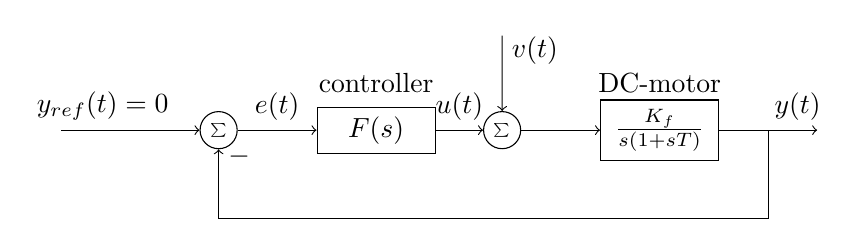
\begin{tikzpicture}[scale = 0.8, node distance=20mm, block/.style={rectangle, draw, minimum width=15mm}, sumnode/.style={circle, draw, inner sep=2pt}]

\node[coordinate] (refinput) {};
\node[sumnode, right of=refinput, node distance=20mm] (sumerr) {\tiny $\sum$};
\node[block, right of=sumerr] (controller) {$F(s)$};
\node[above of=controller, node distance=6mm] {controller};
\node[sumnode, right of=controller, node distance=16mm] (sum) {\tiny $\sum$};
\node[block, right of=sum, node distance=20mm] (tank) {$\frac{K_f}{s(1+sT)}$};
\node[above of=tank, node distance=6mm] {DC-motor};
\node[coordinate, right of=tank, node distance=20mm] (output) {};
\node[coordinate, above of=sum, node distance=12mm] (disturbance) {};

\draw[->] (refinput) -- node[above, pos=0.3] {$y_{ref}(t)=0$} (sumerr);
\draw[->] (sumerr) -- node[above] {$e(t)$} (controller);
\draw[->] (controller) -- node[above] {$u(t)$} (sum);
\draw[->] (sum) -- node[above] {} (tank);
\draw[->] (tank) -- node[coordinate] (measure) {} node[above, pos=0.8] {$y(t)$} (output);
\draw[->] (disturbance) -- node[right, pos=0.2] {$v(t)$} (sum);
\draw[->] (measure) -- ++(0,-14mm) -| node[right, pos=0.95] {$-$} (sumerr);


\end{tikzpicture}
\end{center}

\item The closed-loop system
\[ Y(s) = G_c(s) Y_{ref}(s) + G_d(s) D(s) \] is found by block-diagram calculations to be
\[ Y(s) = \frac{\frac{K_f}{s(1+sT)}F(s)}{1 + \frac{K_f}{s(1+sT)}F(s)}Y_{ref}(s) + 
                    \frac{\frac{K_f}{s(1+sT)}}{1 + \frac{K_f}{s(1+sT)}F(s)}D(s)\]
\[ Y(s) = \frac{K_f F(s)}{s(1+sT) + K_fF(s)}Y_{ref}(s) + \frac{K_f}{s(1+sT) + K_fF(s)} D(s). \]
With proportional controller \( F(s) = K \)
\[ Y(s) = \frac{K_f K}{s(1+sT) + K_fK}Y_{ref}(s) + \frac{K_f}{s(1+sT) + K_fK} D(s). \]
The characteristic polynomial is
\[ s^2 + \frac{1}{T}s + \frac{K_fK}{T} \] and the poles are the roots of this polynomial
\[ s = -\frac{1}{2T} ( 1 \pm \sqrt{1 - 4K_fKT} ). \]
Note that for high gain (\( K \) large) we get a oscillatory closed-loop system. This is a common effect of systems with proportional control.
\item Determine the final values of the output signal, i.e.
\[ \lim_{t \to \infty} y(t) \]
for the two cases
\begin{enumerate}
\item The reference signal $y_{ref}(t)$ is a unit step \( Y_{ref}(s) = \frac{1}{s}\)  and there is no disturbance $d(t)=0$.
\[  \lim_{t \to \infty} y(t) &= \lim_{s \to 0} sY(s) = \lim_{s \to 0} s\frac{K_f K}{s(1+sT) + K_fK}\frac{1}{s} = 1 \]
\item The reference signal is zero and the disturbance $d(t)$ is a unit step.
\[\lim_{t \to \infty} y(t) &= \lim_{s \to 0} sY(s) = \lim_{s \to 0} s\frac{K_f}{s(1+sT) + K_fK}\frac{1}{s} = \frac{1}{K}.\]
Note that with higher gain $K$ we get better disturbance rejection, but we are not able to completety eliminate the disturbance. This is common when only P-control is used.
\end{enumerate}
\item Final value of the control error \(e(t)\) when the reference signal is a step. We have 
\begin{equation*}
\begin{split}
E(s) &= Y_{ref}(s) - Y(s) = \frac{1}{s^2} - \frac{K_fK}{s(1+sT) + K_fK} \frac{1}{s^2} = \frac{s(1+sT) + K_fK - K_f_k}{\left(s(1+sT) + K_fK\right)s^2}\\
&= \frac{1 + sT}{\left(s(1+sT) + K_fK\right)s}
\end{split}
\end{equation*}
so
\[ \lim_{t\to\infty} e(t) = \lim_{s\to 0} s \frac{1 + sT}{\left(s(1+sT) + K_fK\right)s} = \frac{1}{K_fK}. \]
\end{enumerate}
% Emacs 24.5.1 (Org mode 8.2.10)
\end{document}